\documentclass{article}

\usepackage{graphicx}
\usepackage{tikz}
\usepackage{tikzsymbols}
\usetikzlibrary{calc,patterns,shapes.geometric}
\pagestyle{empty}
\usepackage[margin=0pt]{geometry}
\geometry{papersize={14in,12in}}

\def\centerarc[#1](#2)(#3:#4:#5){\draw[#1] ($(#2)+({#5*cos(#3)},{#5*sin(#3)})$) arc (#3:#4:#5);}

\begin{document}
	\begin{figure}
		\centering
		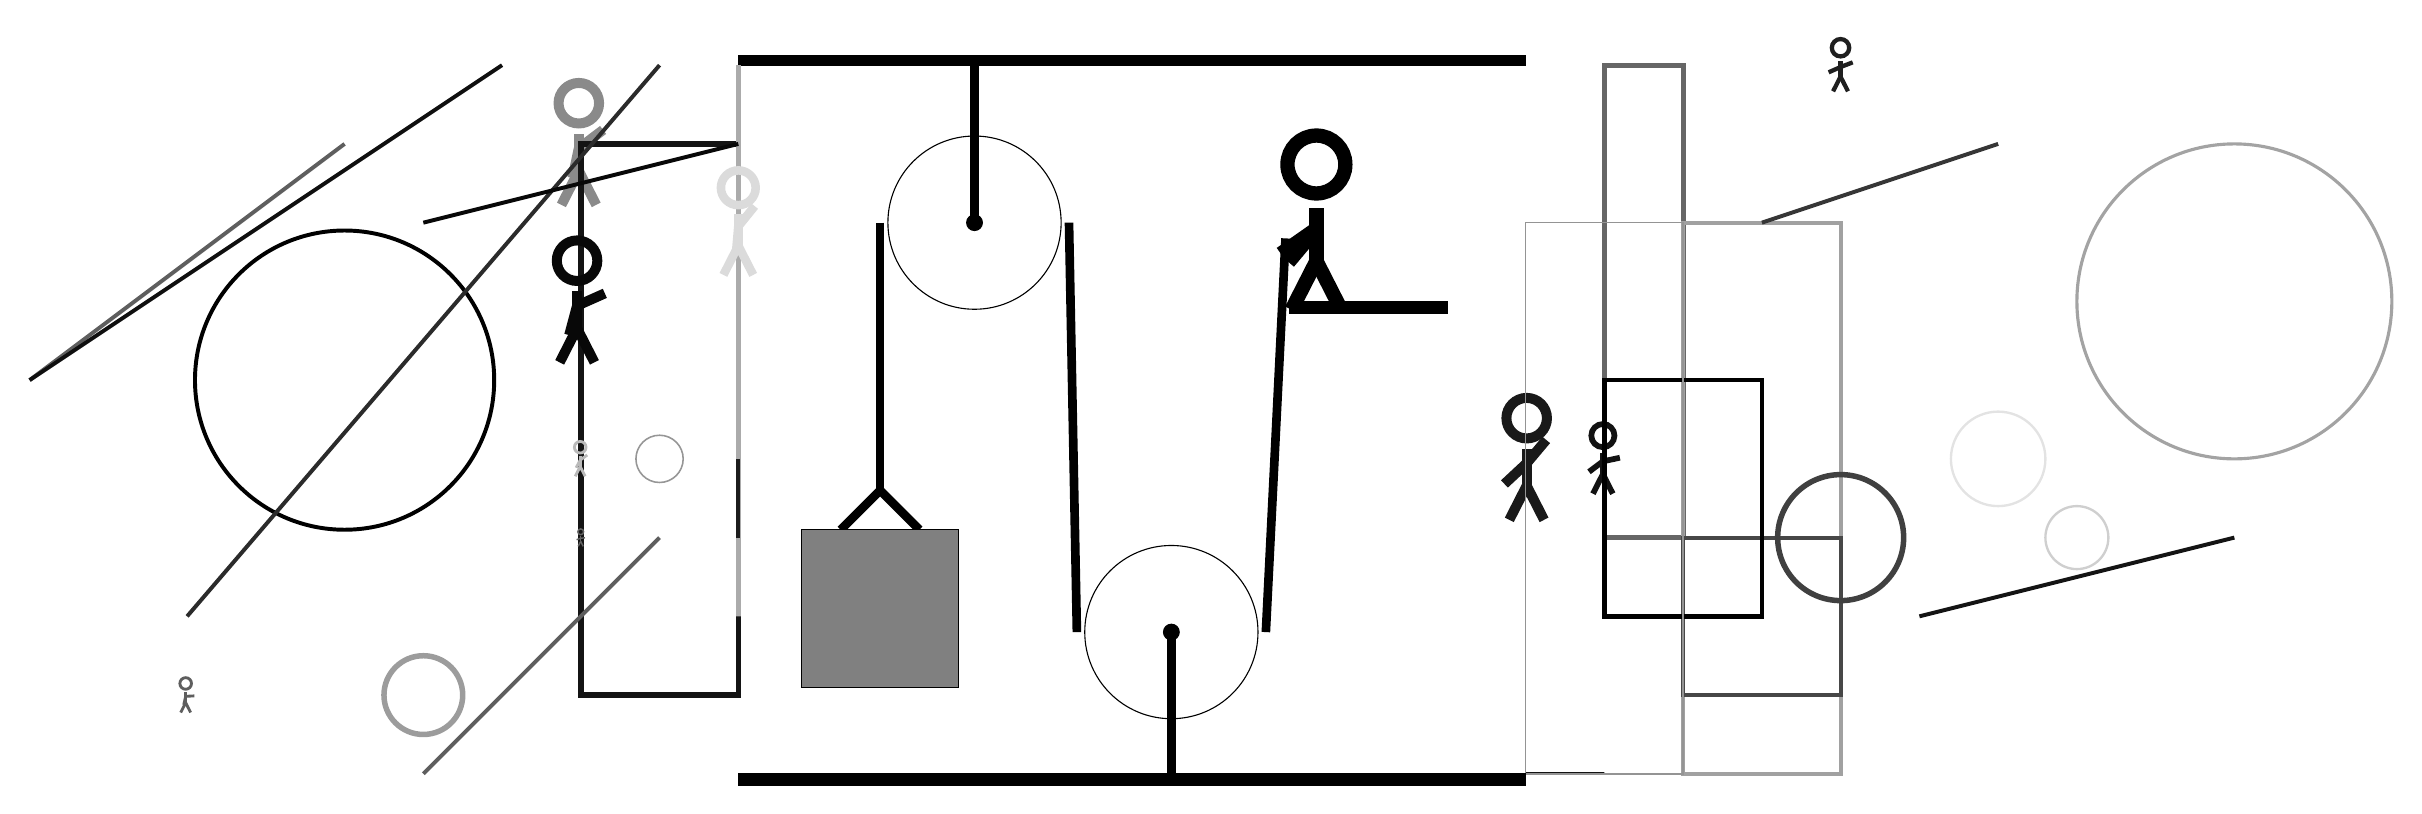
\begin{tikzpicture}
			%%%%% START %%%%%
			
			\draw[fill=black] (-2, 9) rectangle (8, 9.125);
			
			\draw (3.5, 1.8) circle (1.1);
			\draw[fill=black] (3.5, 1.8) circle (0.1);
			\draw[line width=1.1mm] (3.5, 1.8) -- (3.5, 0);
			
			\draw (1, 7) circle (1.1);
			\draw[fill=black] (1, 7) circle (0.1);
			\draw[line width=1.1mm] (1, 9) -- (1, 7);
			
			\draw[line width=1.1mm](-0.7, 3.1) --  (-0.2, 3.6) -- (0.3, 3.1);
			\draw[fill=black!50] (-1.2, 3.1) rectangle (0.8, 1.1);
			
			\node[line width=0.4mm, color=black!46] at (-4, 8) {\Strichmaxerl[7][78][37]};
			
			\draw[line width=0.6mm, color=black!60] (9, 3) rectangle (10, 9);
			\draw [line width=0.5mm, color=black!100](-7, 5) circle (1.9);
			\draw[line width=0.7mm, color=black!92] (-4, 1) rectangle (-2, 8);
			\node[line width=0.4mm, color=black!27] at (-4, 4) {\Strichmaxerl[2][62][36]};
			\draw [line width=0.7mm, color=black!39](-6, 1) circle (0.5);
			\draw[line width=0.6mm, color=black!33] (-2, 9) rectangle (-2, 2);
			
			\draw[line width=0.5mm, color=black!37] (10, 0) rectangle (12, 7);
			\draw[line width=0.5mm, color=black!72] (10, 1) rectangle (12, 3);
			
			\draw[line width=0.5mm, color=black!63](-3, 3) -- (-6, 0);
			\draw[line width=0.5mm, color=black!92](13, 2) -- (17, 3);
			\node[line width=0.3mm, color=black!63] at (-9, 1) {\Strichmaxerl[2][77][3]};
			\draw [line width=0.4mm, color=black!36](17, 6) circle (2.0);
			\draw[line width=0.4mm, color=black!93] (9, 0) rectangle (8, 0);
			\draw[line width=0.5mm, color=black!83](-3, 9) -- (-9, 2);
			\draw[line width=0.5mm, color=black!97](-6, 7) -- (-2, 8);
			
			\draw [line width=0.7mm, color=black!75](12, 3) circle (0.8);
			
			\node[line width=0.2mm, color=black!90] at (8, 4) {\Strichmaxerl[7][43][50]};
			\draw [line width=0.3mm, color=black!11](14, 4) circle (0.6);
			
			\draw[line width=0.5mm, color=black!79](11, 7) -- (14, 8);
			\draw [line width=0.2mm, color=black!41](-3, 4) circle (0.3);
			\node[line width=0.6mm, color=black!88] at (12, 9) {\Strichmaxerl[3][24][21]};
			\node[line width=0.3mm, color=black!97] at (-4, 6) {\Strichmaxerl[7][75][24]};
			\node[line width=0.6mm, color=black!93] at (9, 4) {\Strichmaxerl[4][37][12]};
			\draw [line width=0.3mm, color=black!19](15, 3) circle (0.4);
			\node[line width=0.6mm, color=black!14] at (-2, 7) {\Strichmaxerl[6][85][51]};
			\node[line width=0.7mm, color=black!61] at (-4, 3) {\Strichmaxerl[1][20][6]};
			\draw[line width=0.6mm, color=black!100] (9, 5) rectangle (11, 2);
			
			\draw[line width=0.5mm, color=black!63](-7, 8) -- (-11, 5);
			\draw[line width=0.2mm, color=black!42] (8, 7) rectangle (10, 0);
			\draw[line width=0.5mm, color=black!94](-5, 9) -- (-11, 5);
			
			\draw[line width=0.5mm, color=black!89](-2, 4) -- (-2, 3);
			
			\draw[line width=1.1mm](-0.2, 7) -- (-0.2, 3.6);
			\centerarc[line width=1.1mm](1, 7)(180:0:1.2000000000000002)
			\draw[line width=1.1mm](2.2, 7) -- (2.3, 1.8);
			\centerarc[line width=1.1mm](3.5, 1.8)(180:360:1.2000000000000002)
			\draw[line width=1.1mm](4.7, 1.8) -- (4.95, 6.8);
			
			\node at (5.3, 7) {\Strichmaxerl[10][35][-130]};
			\draw[fill=black] (5, 6) rectangle (7, 5.85);
			
			\draw[fill=black] (-2, 0) rectangle (8, -0.15);
			
			%%%%% END %%%%%
		\end{tikzpicture}
	\end{figure}	
\end{document}